\appendix

\chapter{Anhang}

\section{Ergänzende Darstellungen zu den Resultaten}

\subsection{Vergleich der topologischen Indizes pro Klasse} \label{sec:compare-ti-classes}

\begin{figure}[H]
    \centering
    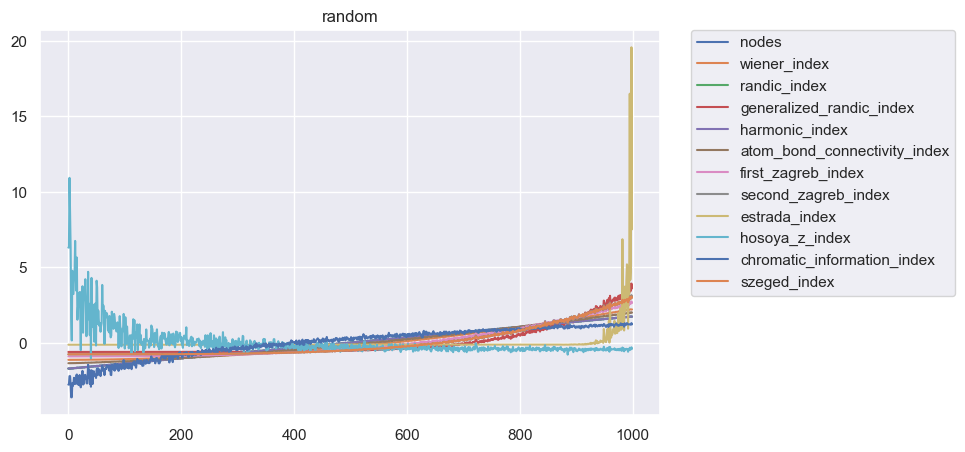
\includegraphics[width=\textwidth]{images/30_results/random-ti-comparison.png}
    \caption{Topologische Indizes der Klasse \mintinline{python3}{random}}
    \label{fig:big-ti-comparison-random}
\end{figure}
\begin{figure}[H]
    \centering
    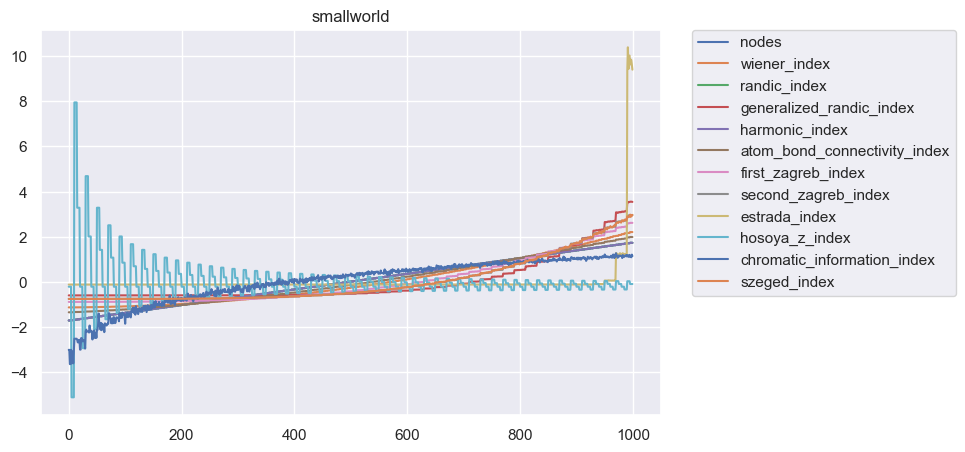
\includegraphics[width=\textwidth]{images/30_results/smallworld-ti-comparison.png}
    \caption{Topologische Indizes der Klasse \mintinline{python3}{smallworld}}
    \label{fig:big-ti-comparison-smallworld}
\end{figure}

\begin{figure}[H]
    \centering
    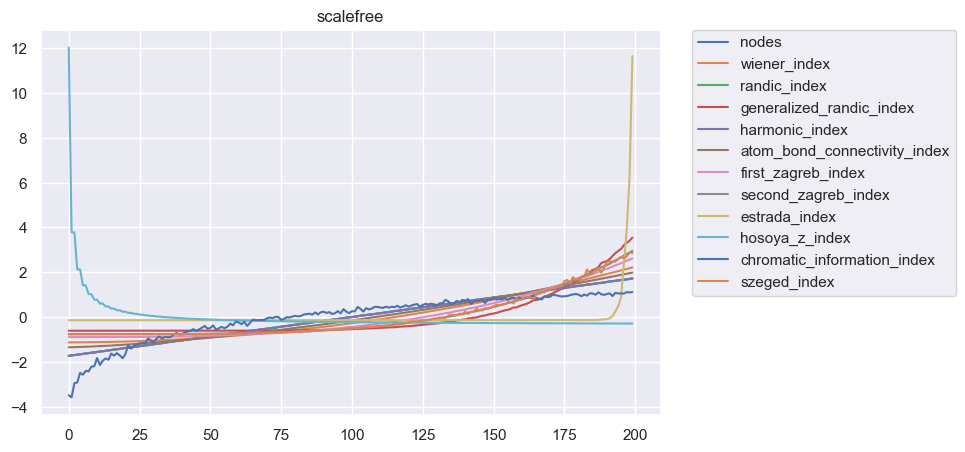
\includegraphics[width=\textwidth]{images/30_results/scalefree-ti-comparison.png}
    \caption{Topologische Indizes der Klasse \mintinline{python3}{scalefree}}
    \label{fig:big-ti-comparison-scalefree}
\end{figure}
\begin{figure}[H]
    \centering
    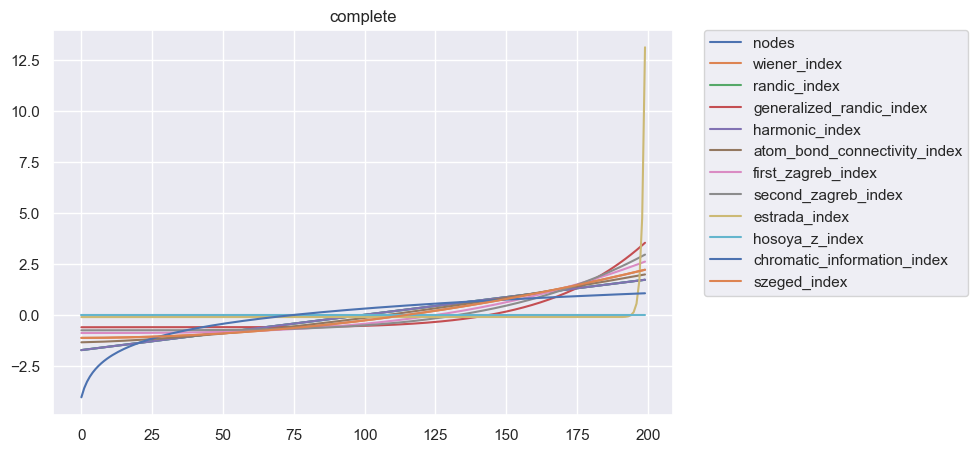
\includegraphics[width=\textwidth]{images/30_results/complete-ti-comparison.png}
    \caption{Topologische Indizes der Klasse \mintinline{python3}{complete}}
    \label{fig:big-ti-comparison-complete}
\end{figure}

\begin{figure}[H]
    \centering
    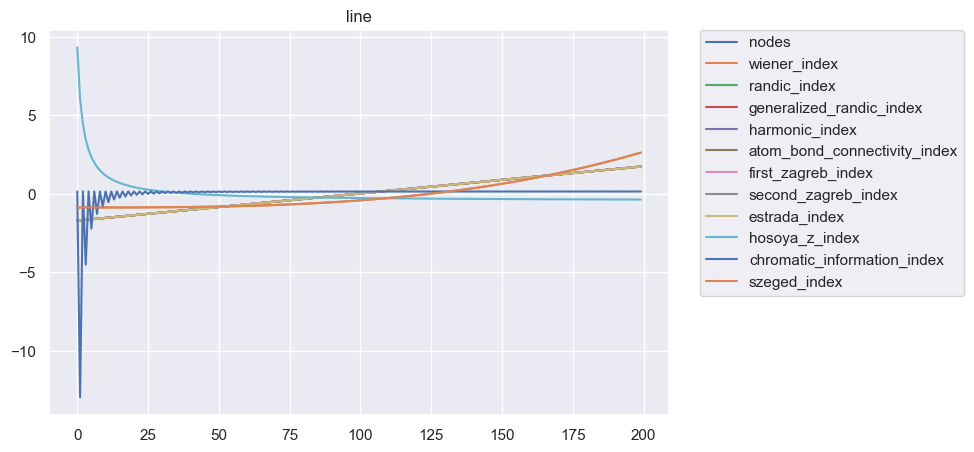
\includegraphics[width=\textwidth]{images/30_results/line-ti-comparison.png}
    \caption{Topologische Indizes der Klasse \mintinline{python3}{line}}
    \label{fig:big-ti-comparison-line}
\end{figure}
\begin{figure}[H]
    \centering
    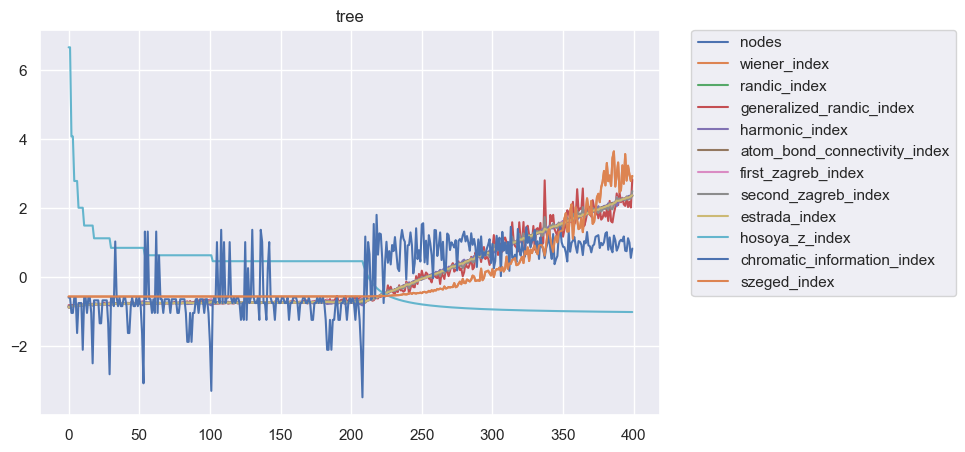
\includegraphics[width=\textwidth]{images/30_results/tree-ti-comparison.png}
    \caption{Topologische Indizes der Klasse \mintinline{python3}{tree}}
    \label{fig:big-ti-comparison-tree}
\end{figure}

\begin{figure}[H]
    \centering
    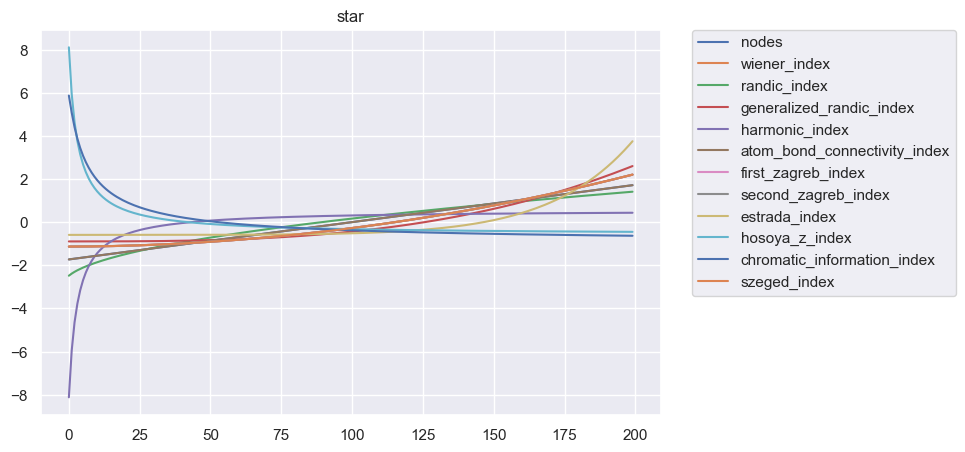
\includegraphics[width=\textwidth]{images/30_results/star-ti-comparison.png}
    \caption{Topologische Indizes der Klasse \mintinline{python3}{star}}
    \label{fig:big-ti-comparison-star}
\end{figure}

\newpage
\subsection{Einzel-Vergleich der topologischen Indizes} \label{sec:correlation-pairs}

\begin{figure}[H]
    \centering
    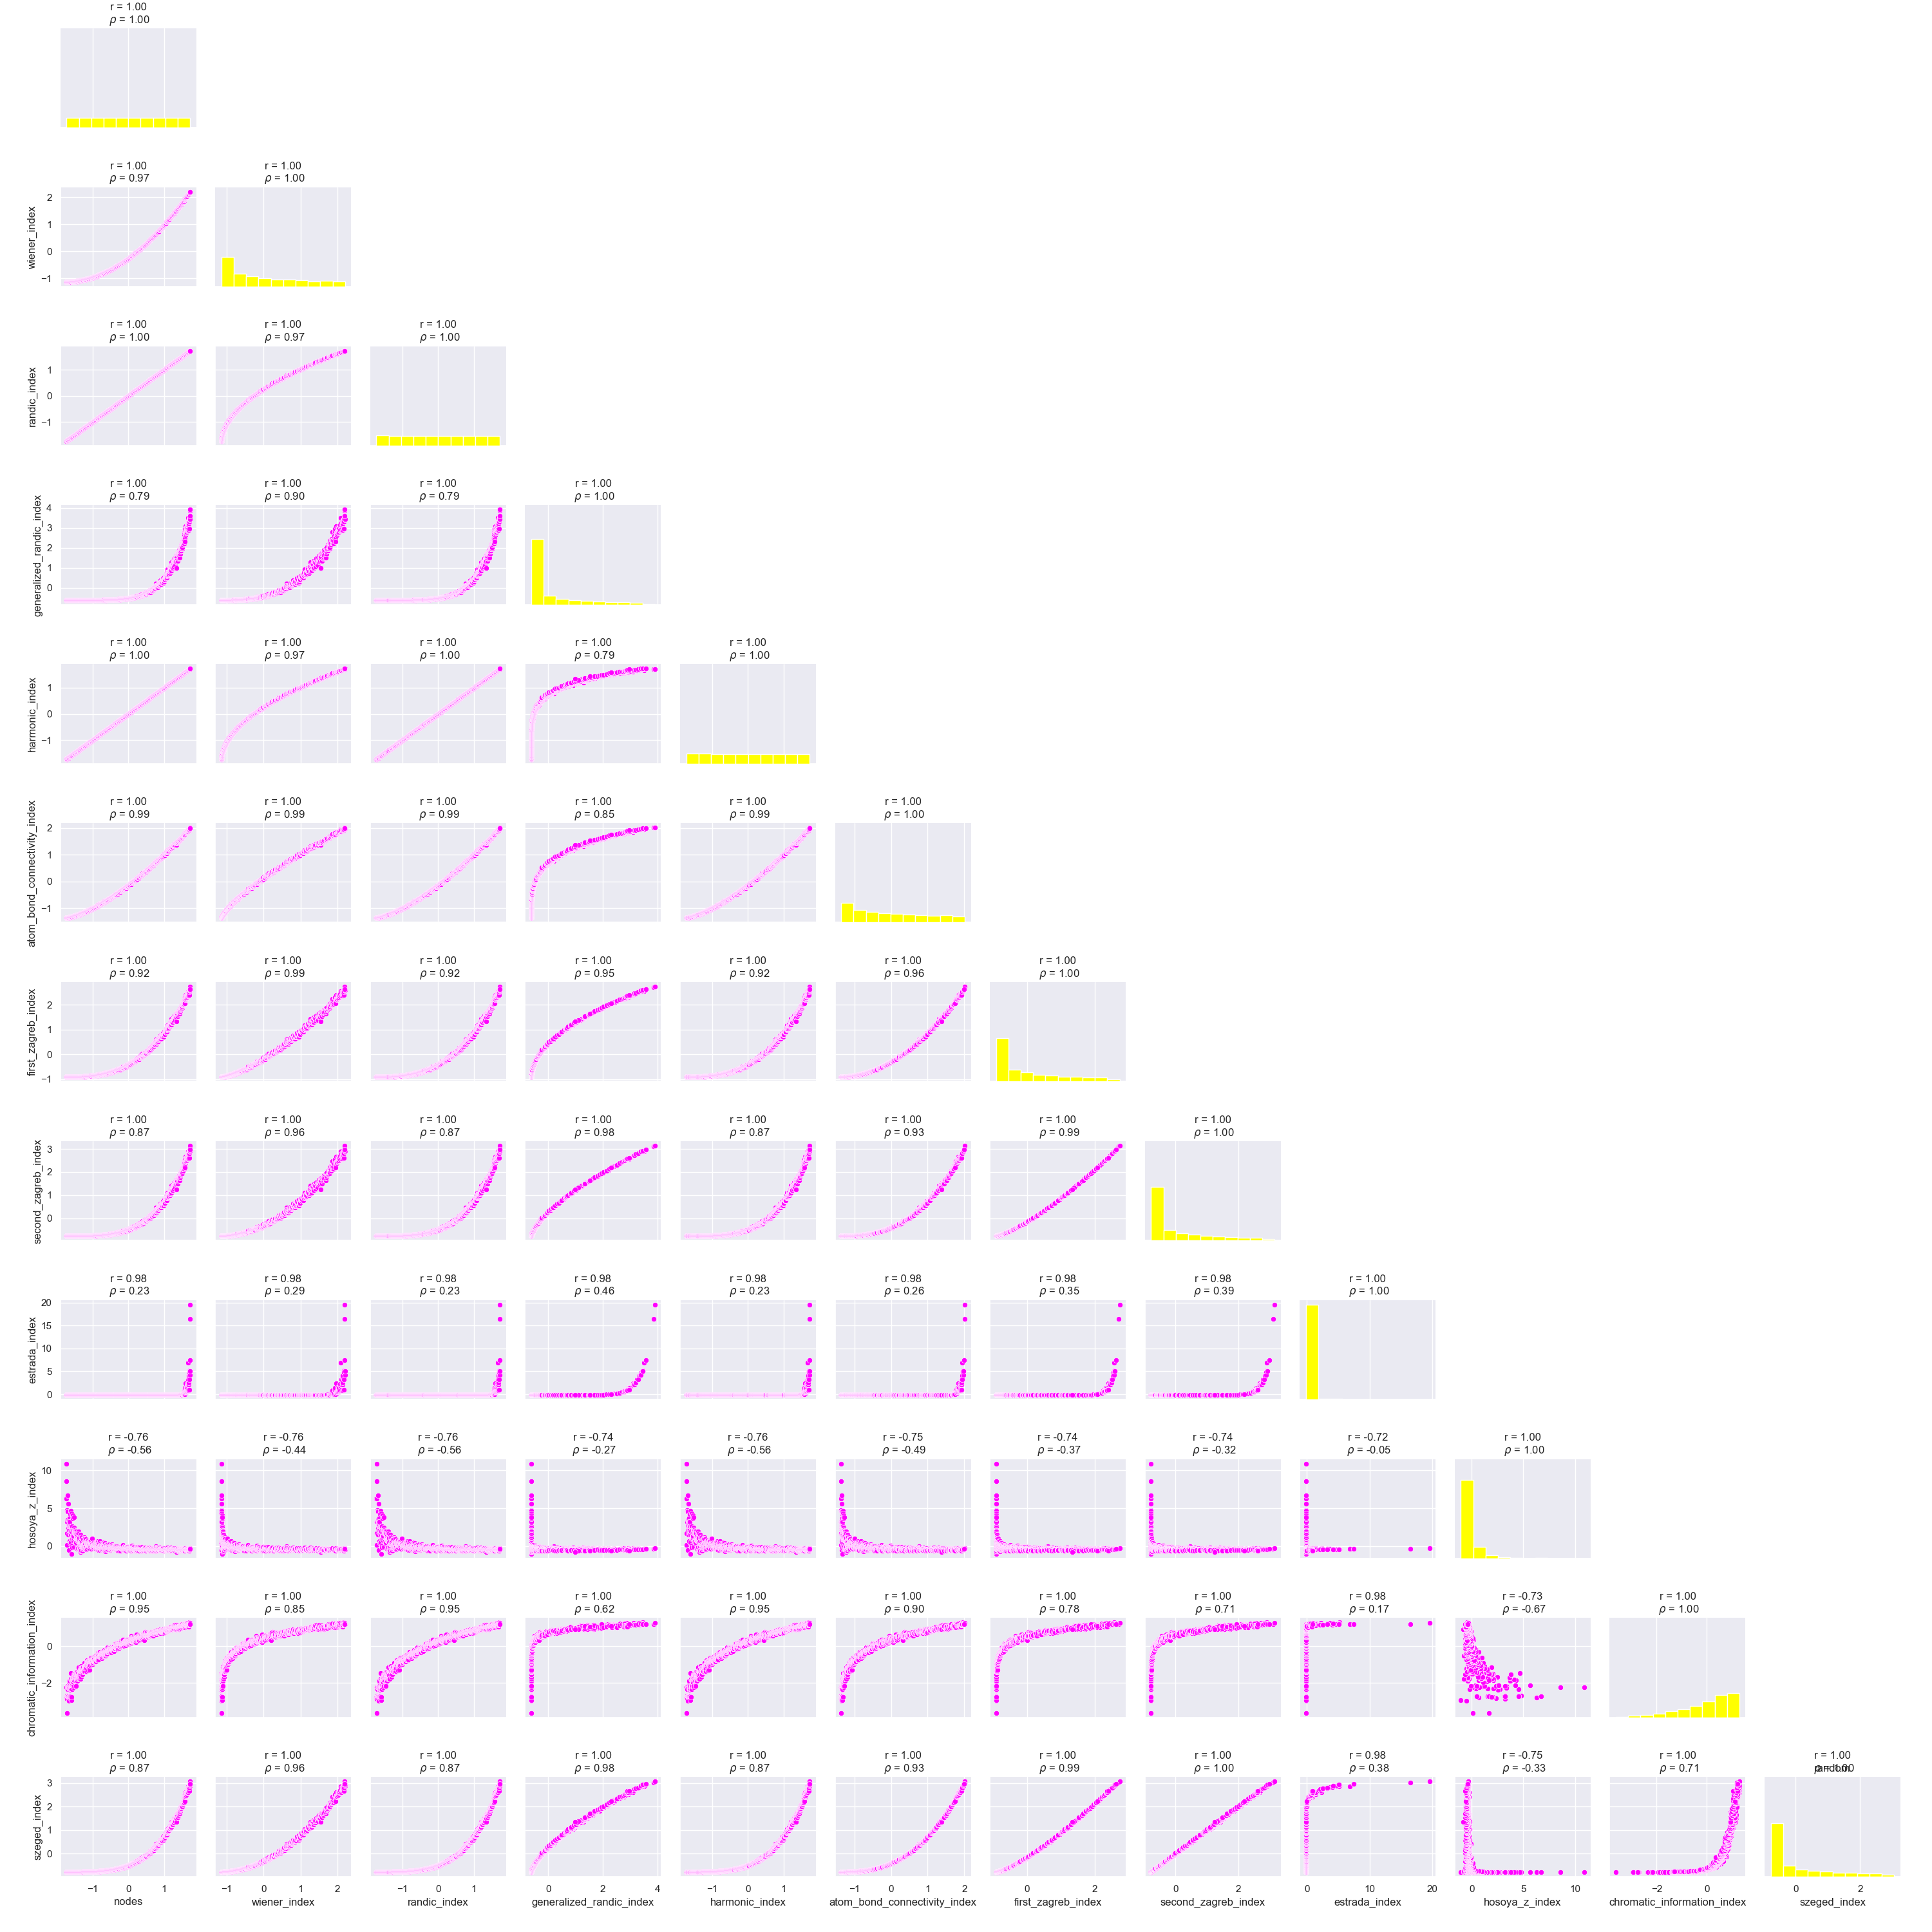
\includegraphics[width=1.2\textwidth]{images/30_results/random-correlation-pairs.png}
    \caption{Einzelne Vergleiche der topologischen Indizes der Klasse \mintinline{python3}{random}}
    \label{fig:correlation-pairs-random}
\end{figure}

\begin{figure}[H]
    \centering
    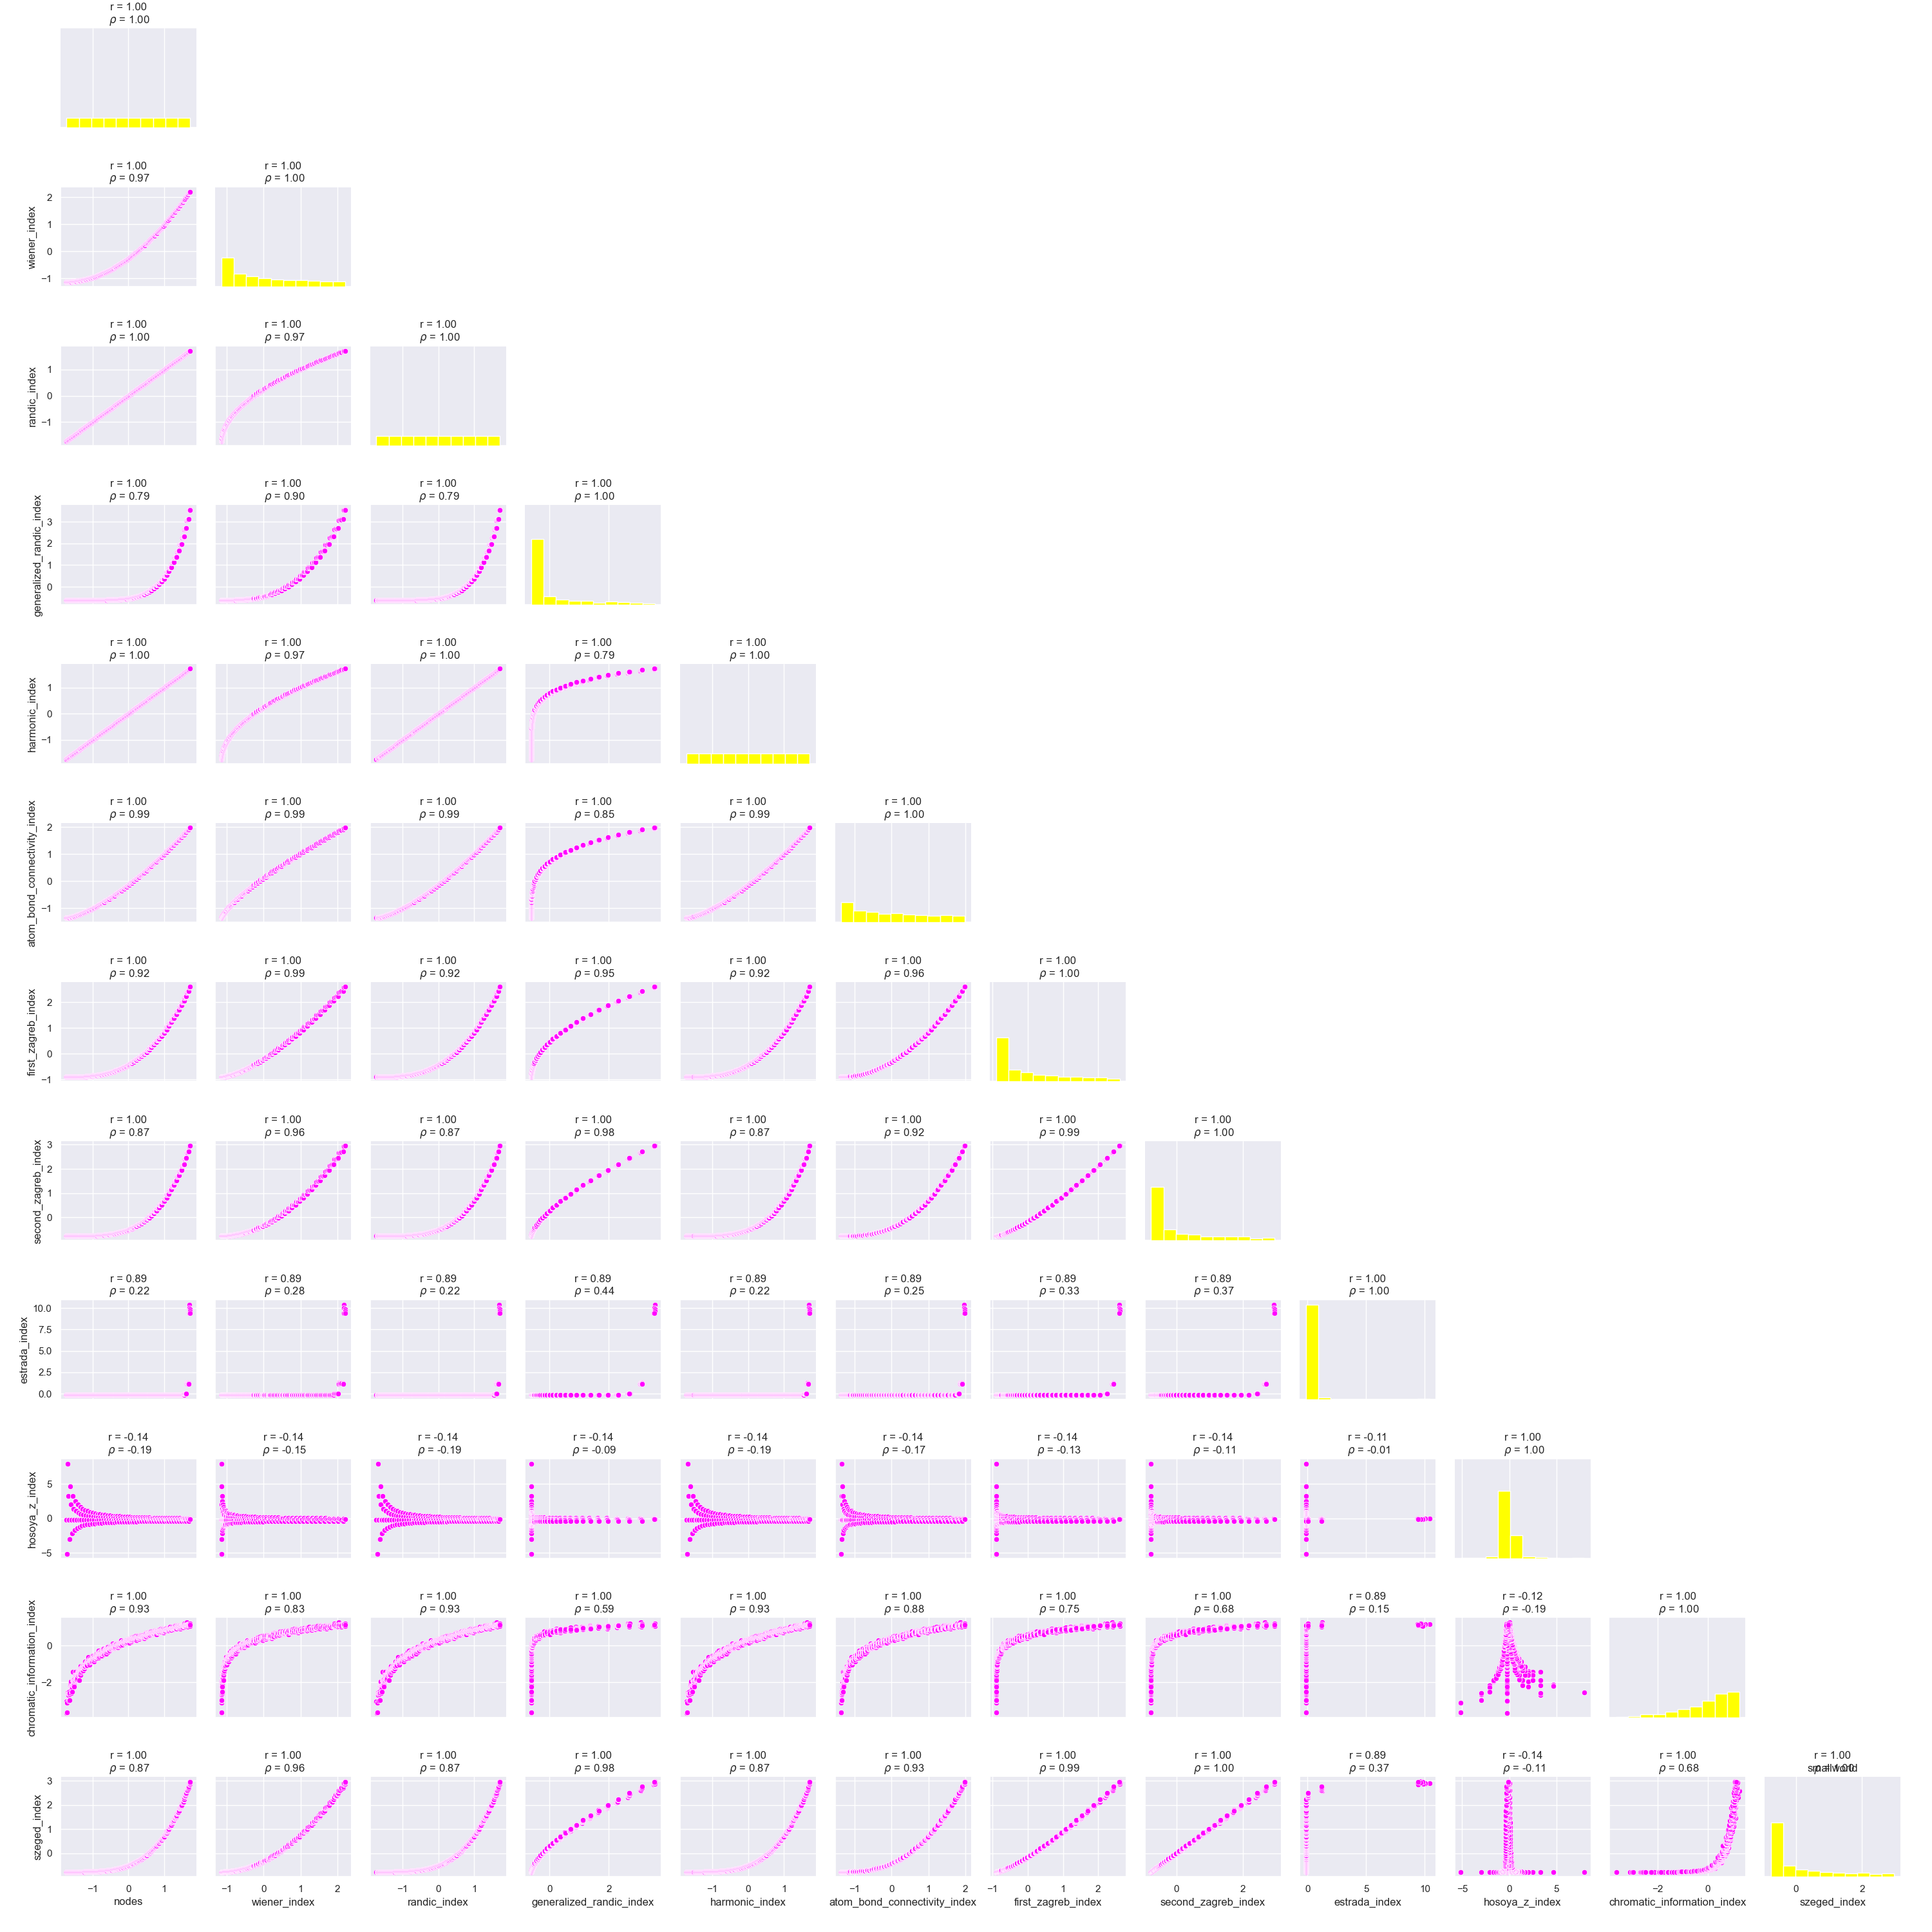
\includegraphics[width=1.2\textwidth]{images/30_results/smallworld-correlation-pairs.png}
    \caption{Einzelne Vergleiche der topologischen Indizes der Klasse \mintinline{python3}{smallworld}}
    \label{fig:correlation-pairs-smallworld}
\end{figure}

\begin{figure}[H]
    \centering
    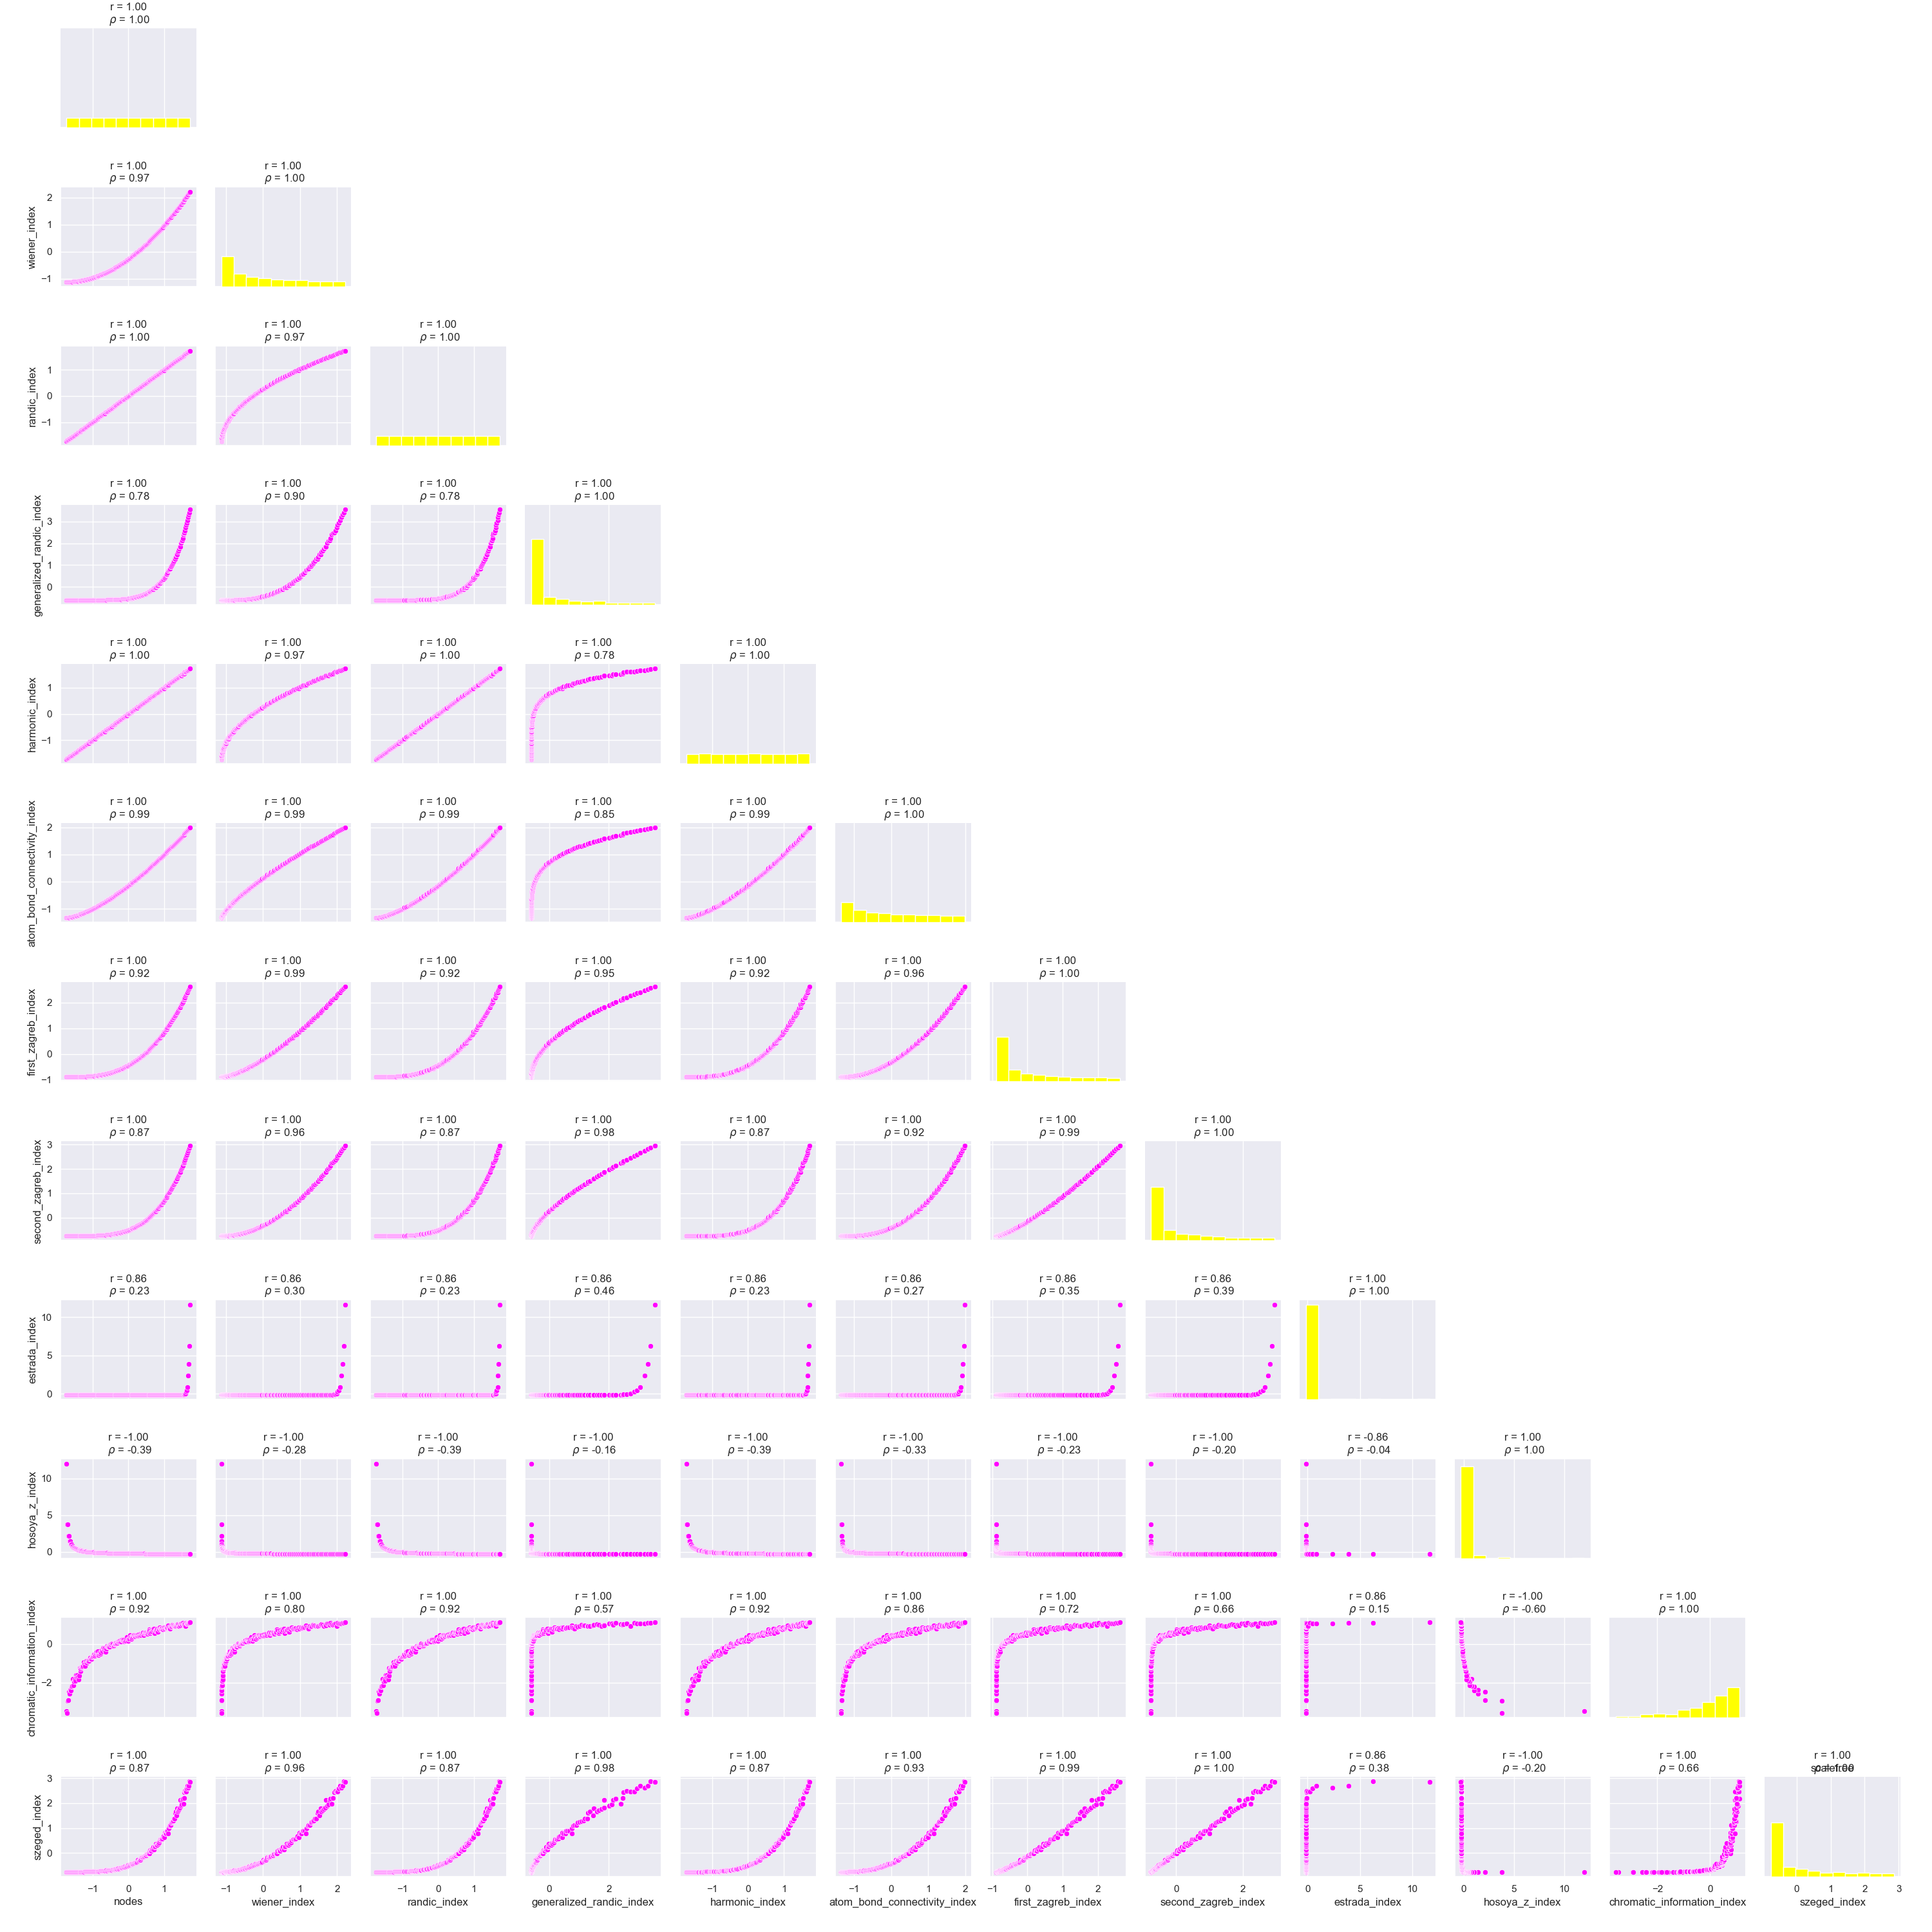
\includegraphics[width=1.2\textwidth]{images/30_results/scalefree-correlation-pairs.png}
    \caption{Einzelne Vergleiche der topologischen Indizes der Klasse \mintinline{python3}{scalefree}}
    \label{fig:correlation-pairs-scalefree}
\end{figure}

\begin{figure}[H]
    \centering
    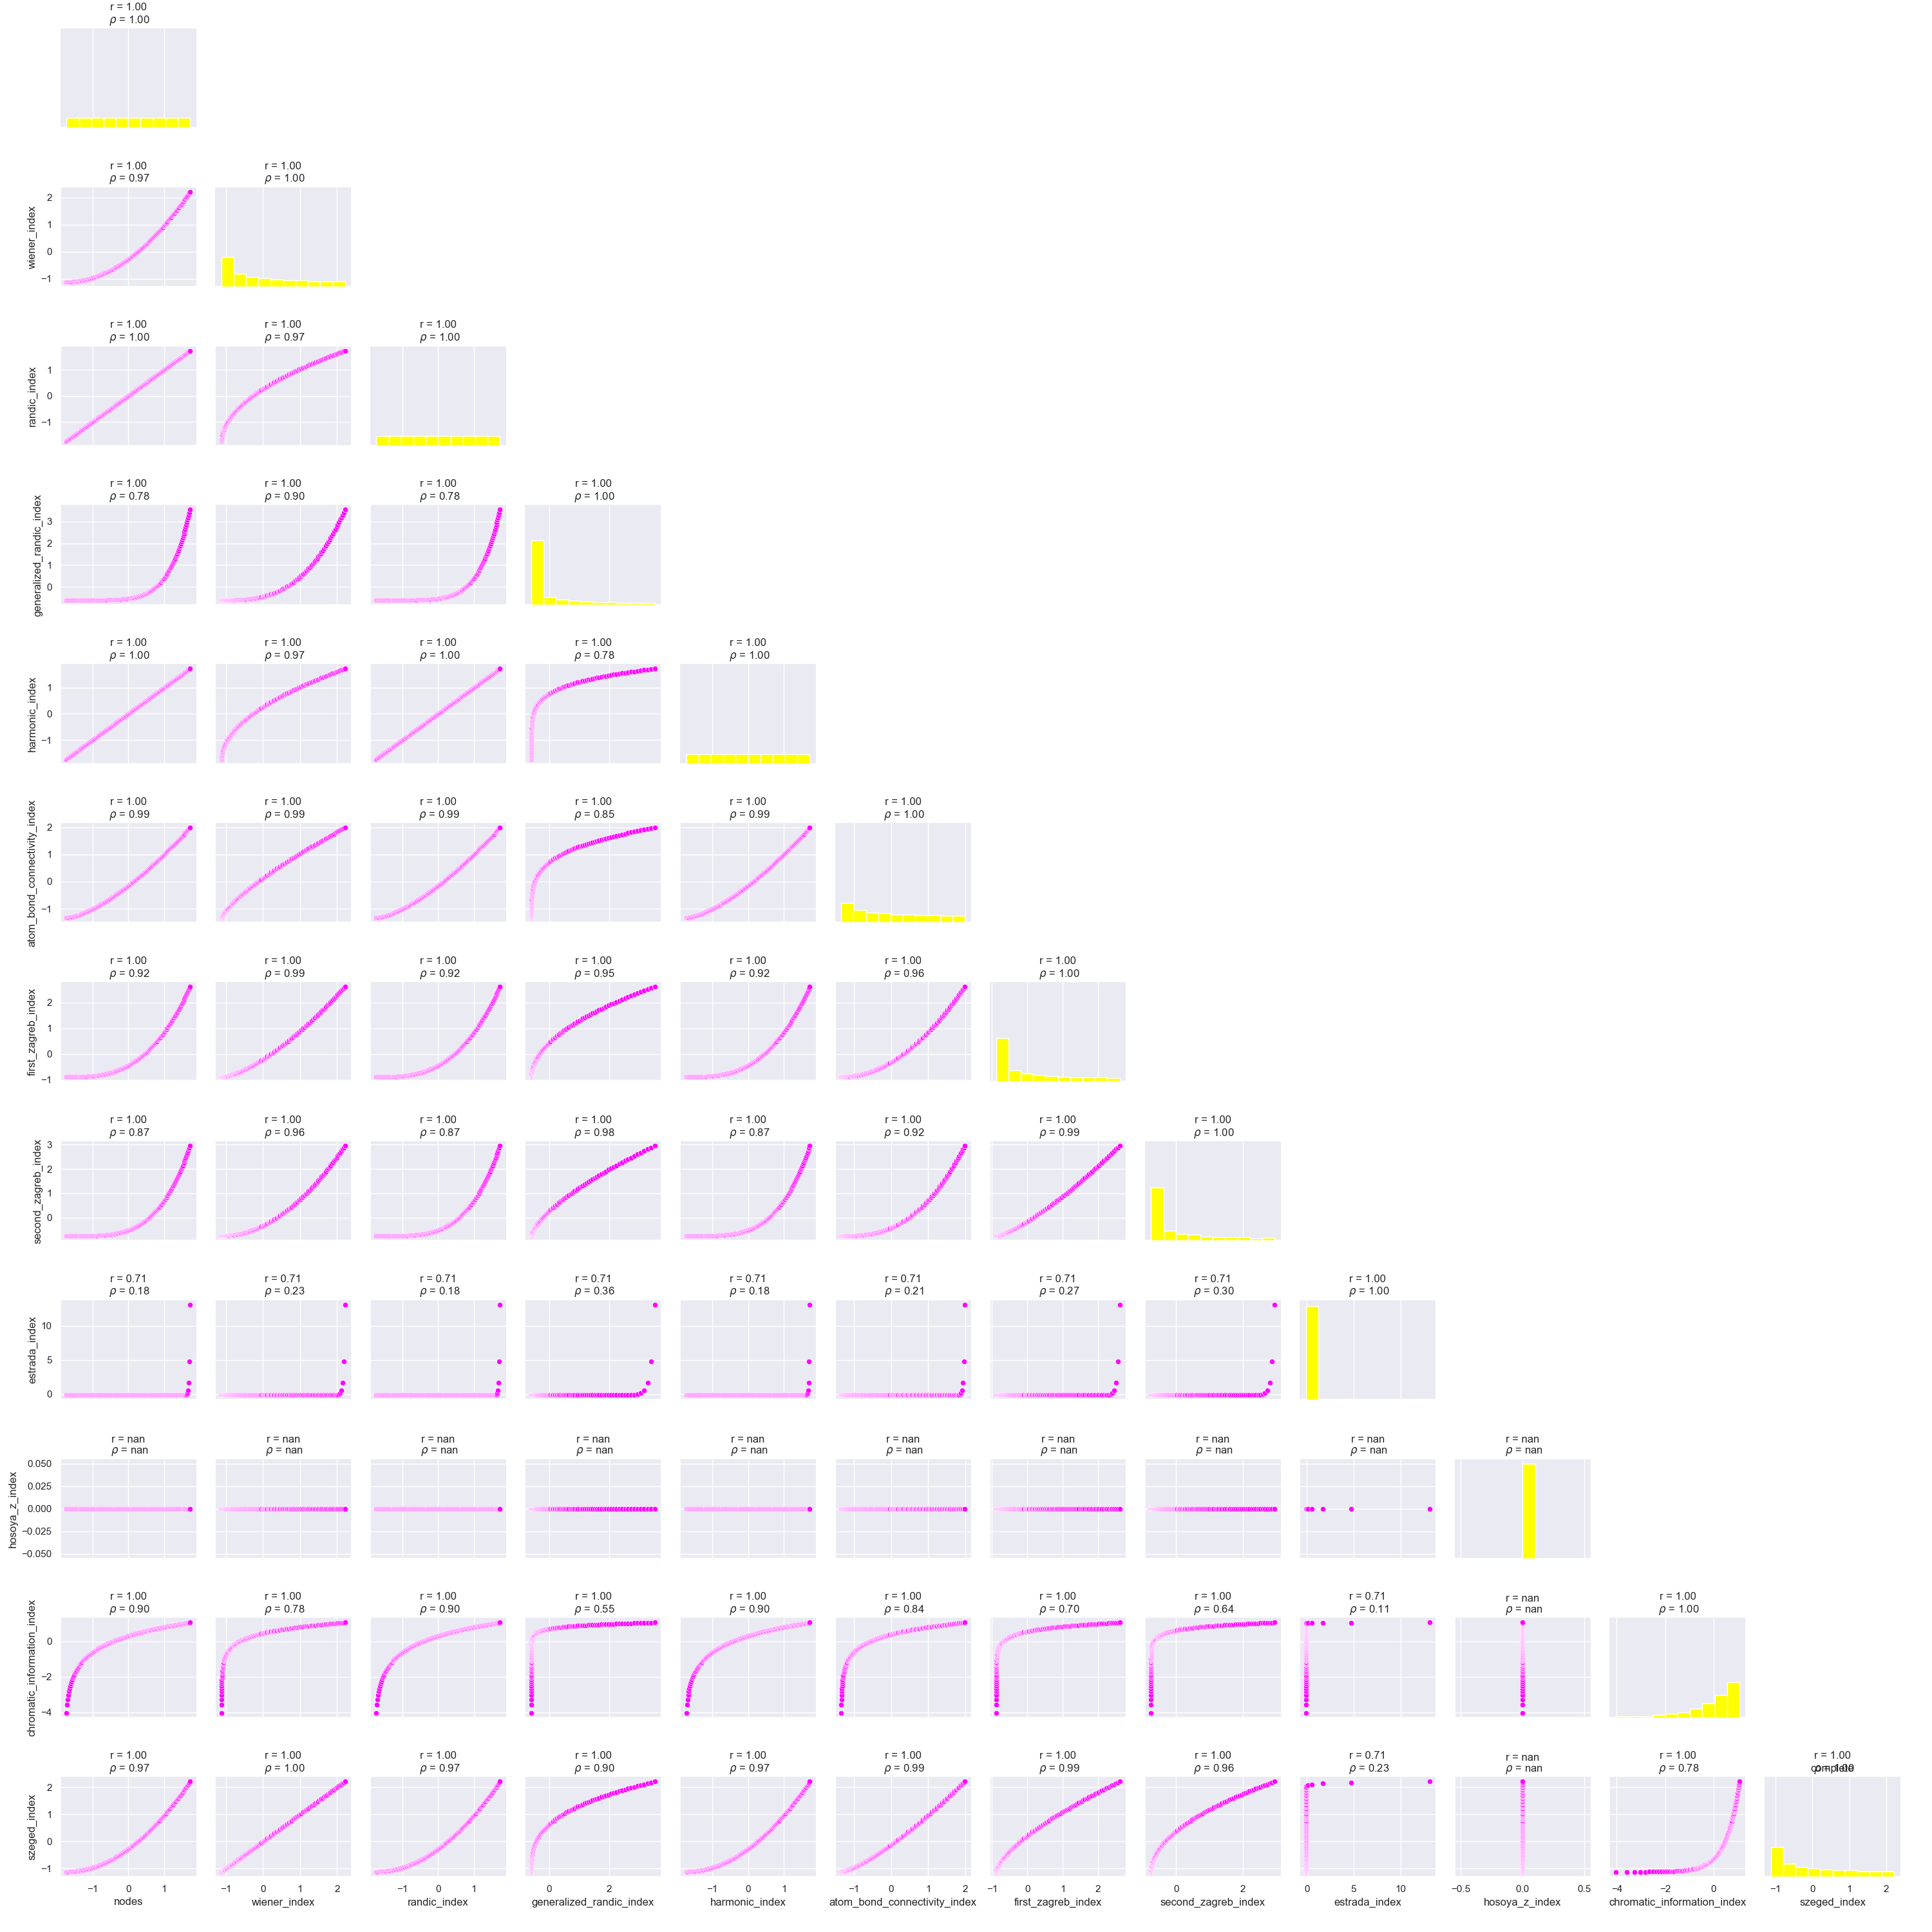
\includegraphics[width=1.2\textwidth]{images/30_results/complete-correlation-pairs.png}
    \caption{Einzelne Vergleiche der topologischen Indizes der Klasse \mintinline{python3}{complete}}
    \label{fig:correlation-pairs-complete}
\end{figure}

\begin{figure}[H]
    \centering
    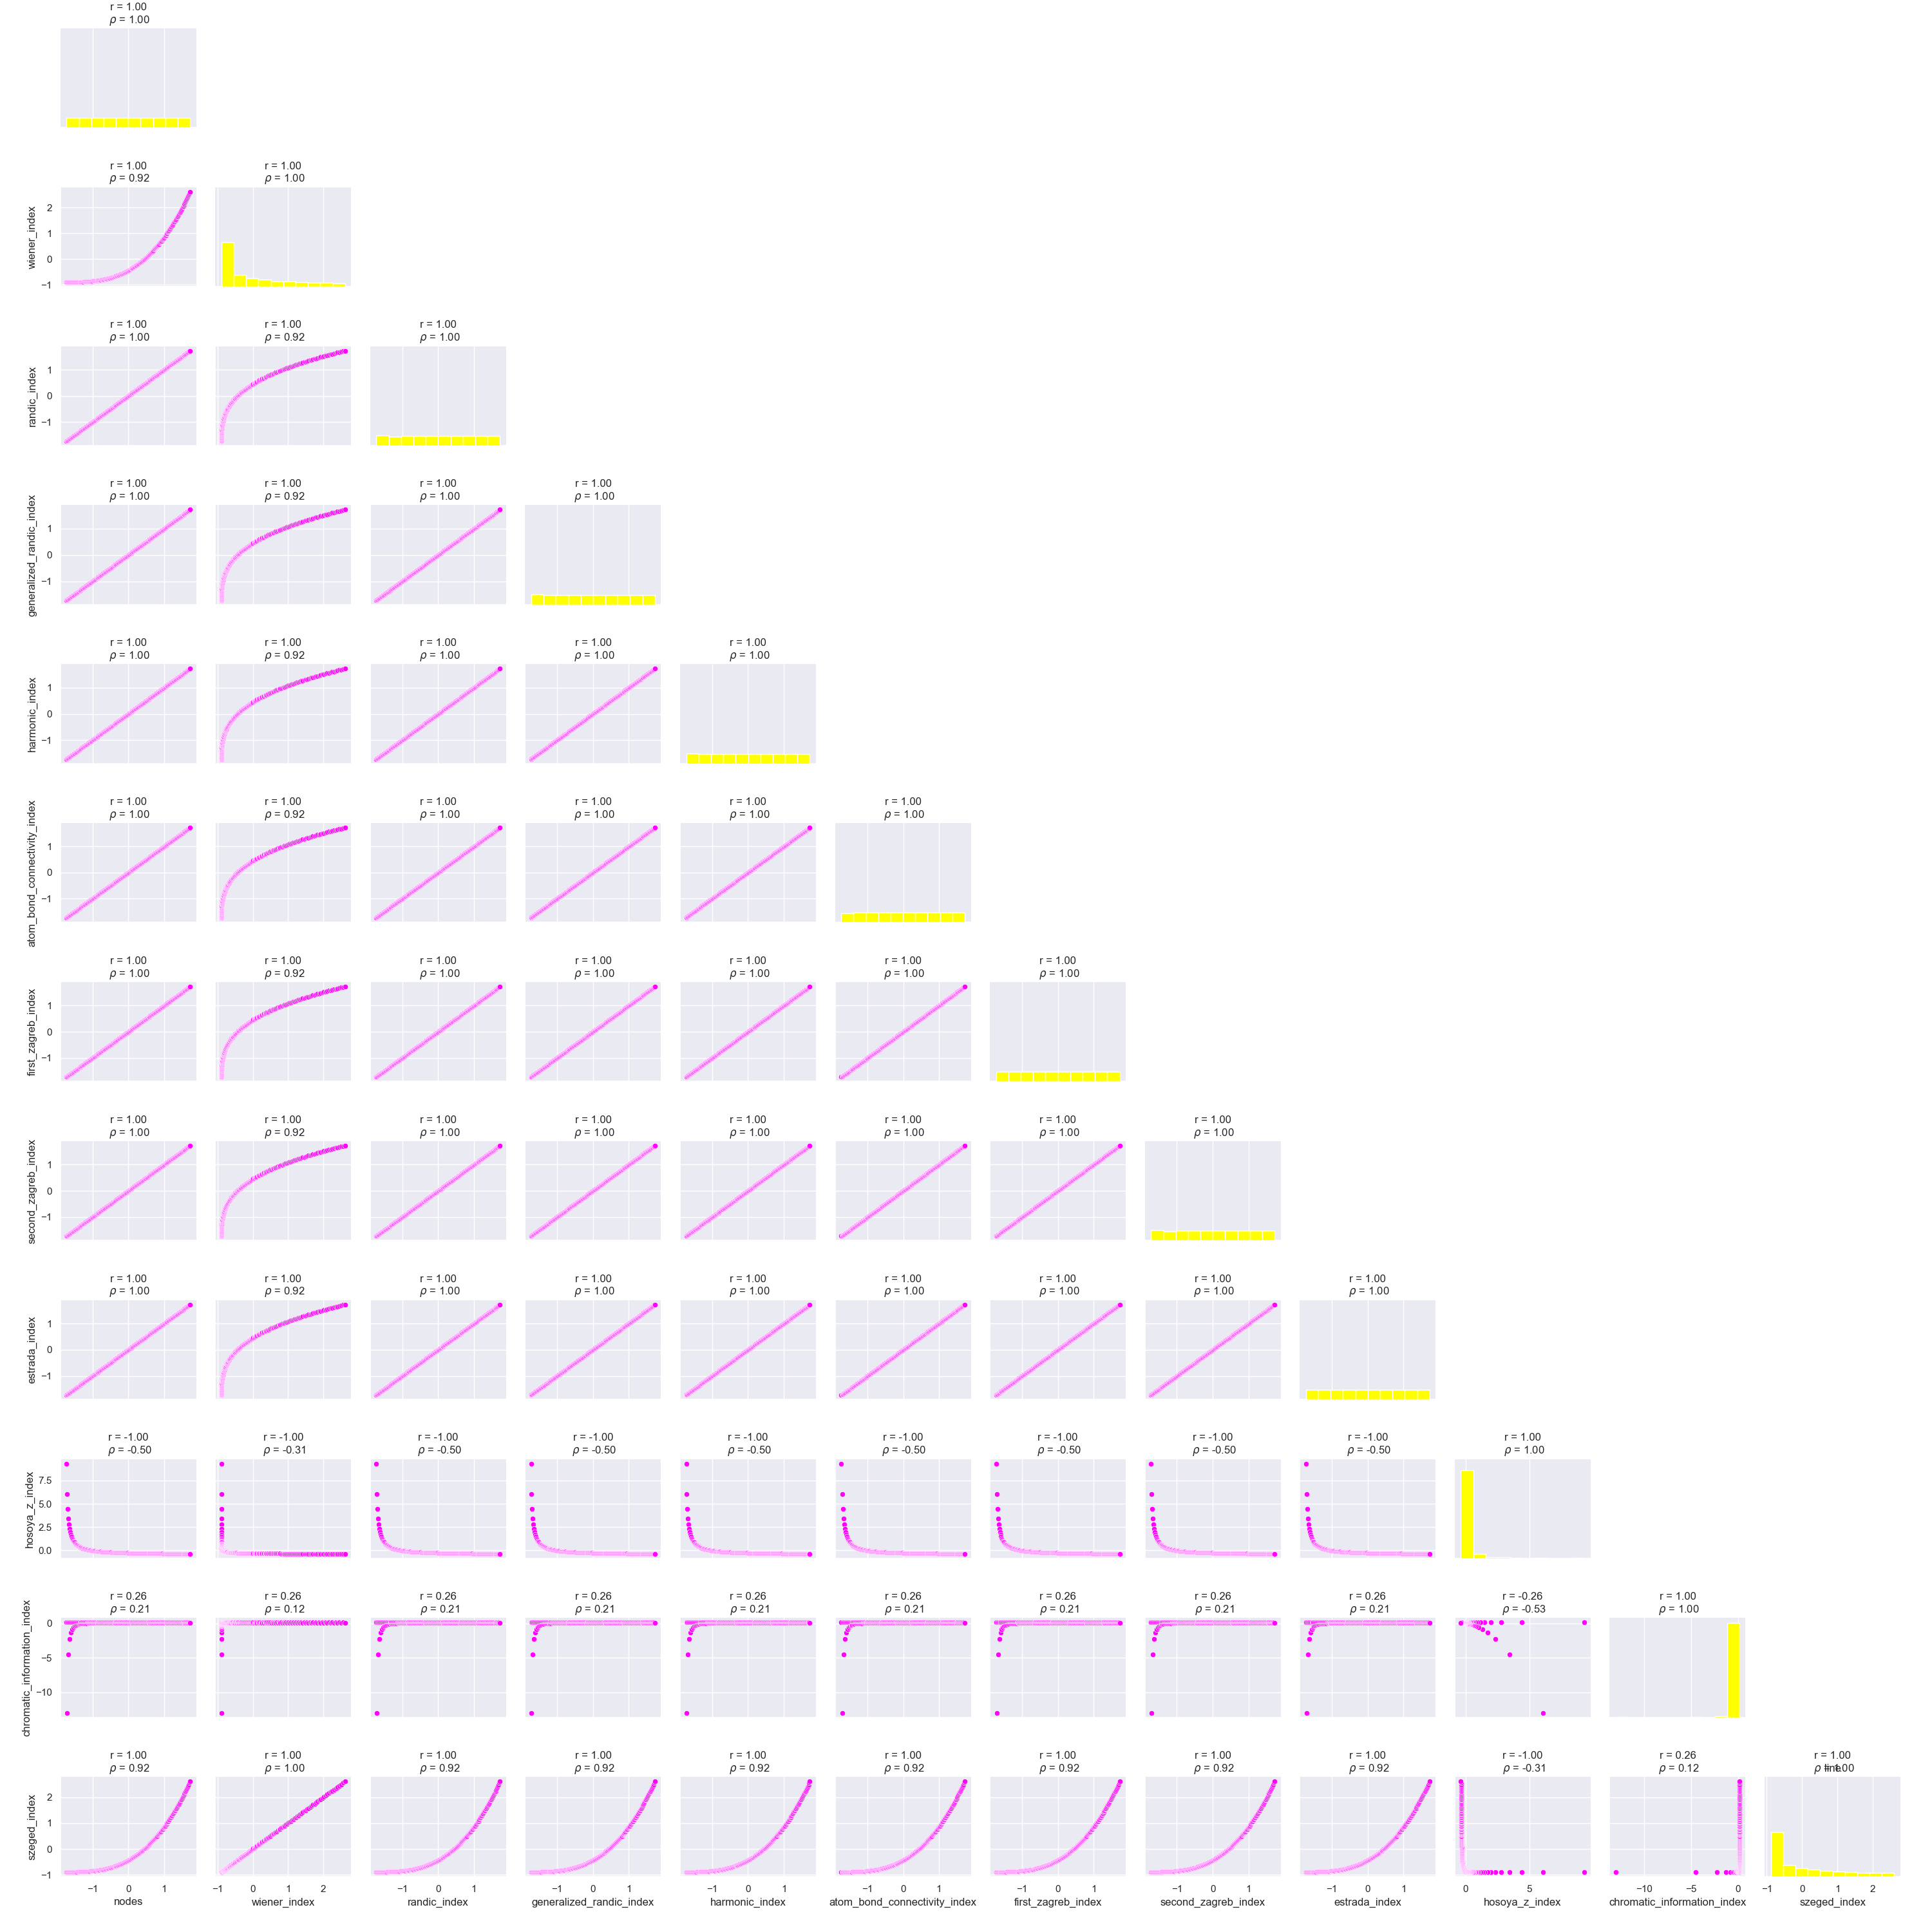
\includegraphics[width=1.2\textwidth]{images/30_results/line-correlation-pairs.png}
    \caption{Einzelne Vergleiche der topologischen Indizes der Klasse \mintinline{python3}{line}}
    \label{fig:correlation-pairs-line}
\end{figure}

\begin{figure}[H]
    \centering
    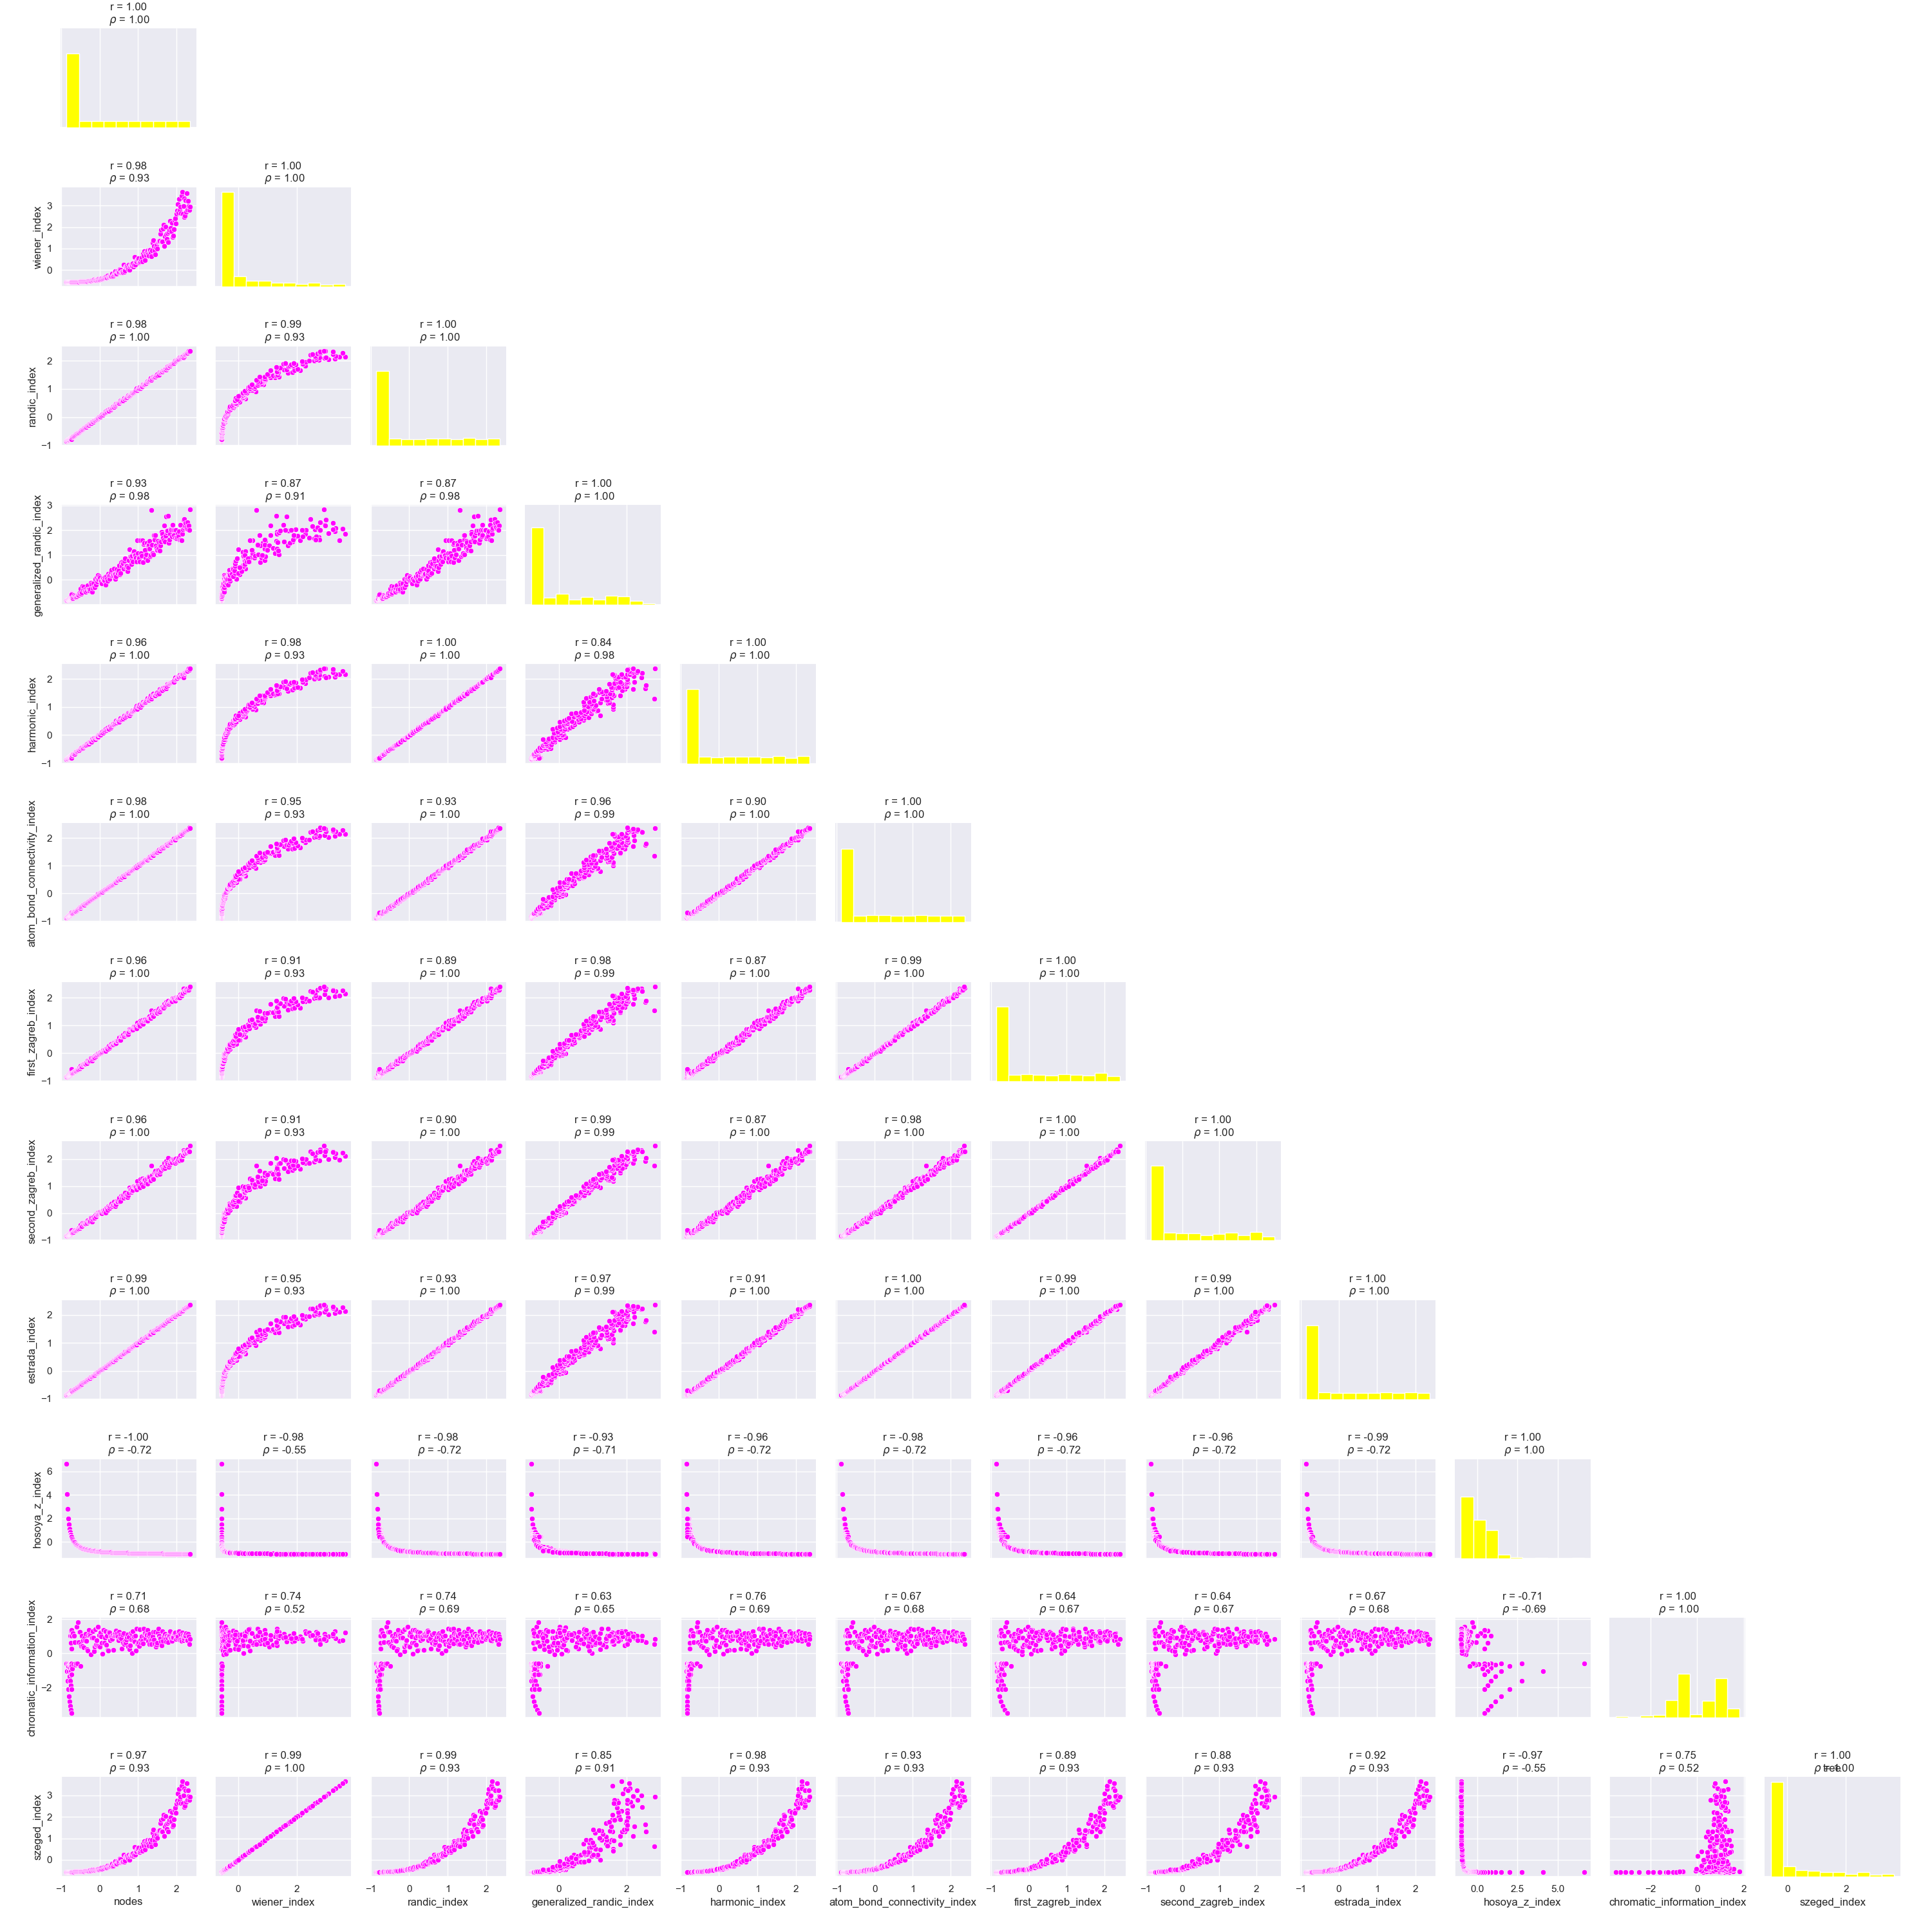
\includegraphics[width=1.2\textwidth]{images/30_results/tree-correlation-pairs.png}
    \caption{Einzelne Vergleiche der topologischen Indizes der Klasse \mintinline{python3}{tree}}
    \label{fig:correlation-pairs-tree}
\end{figure}

\begin{figure}[H]
    \centering
    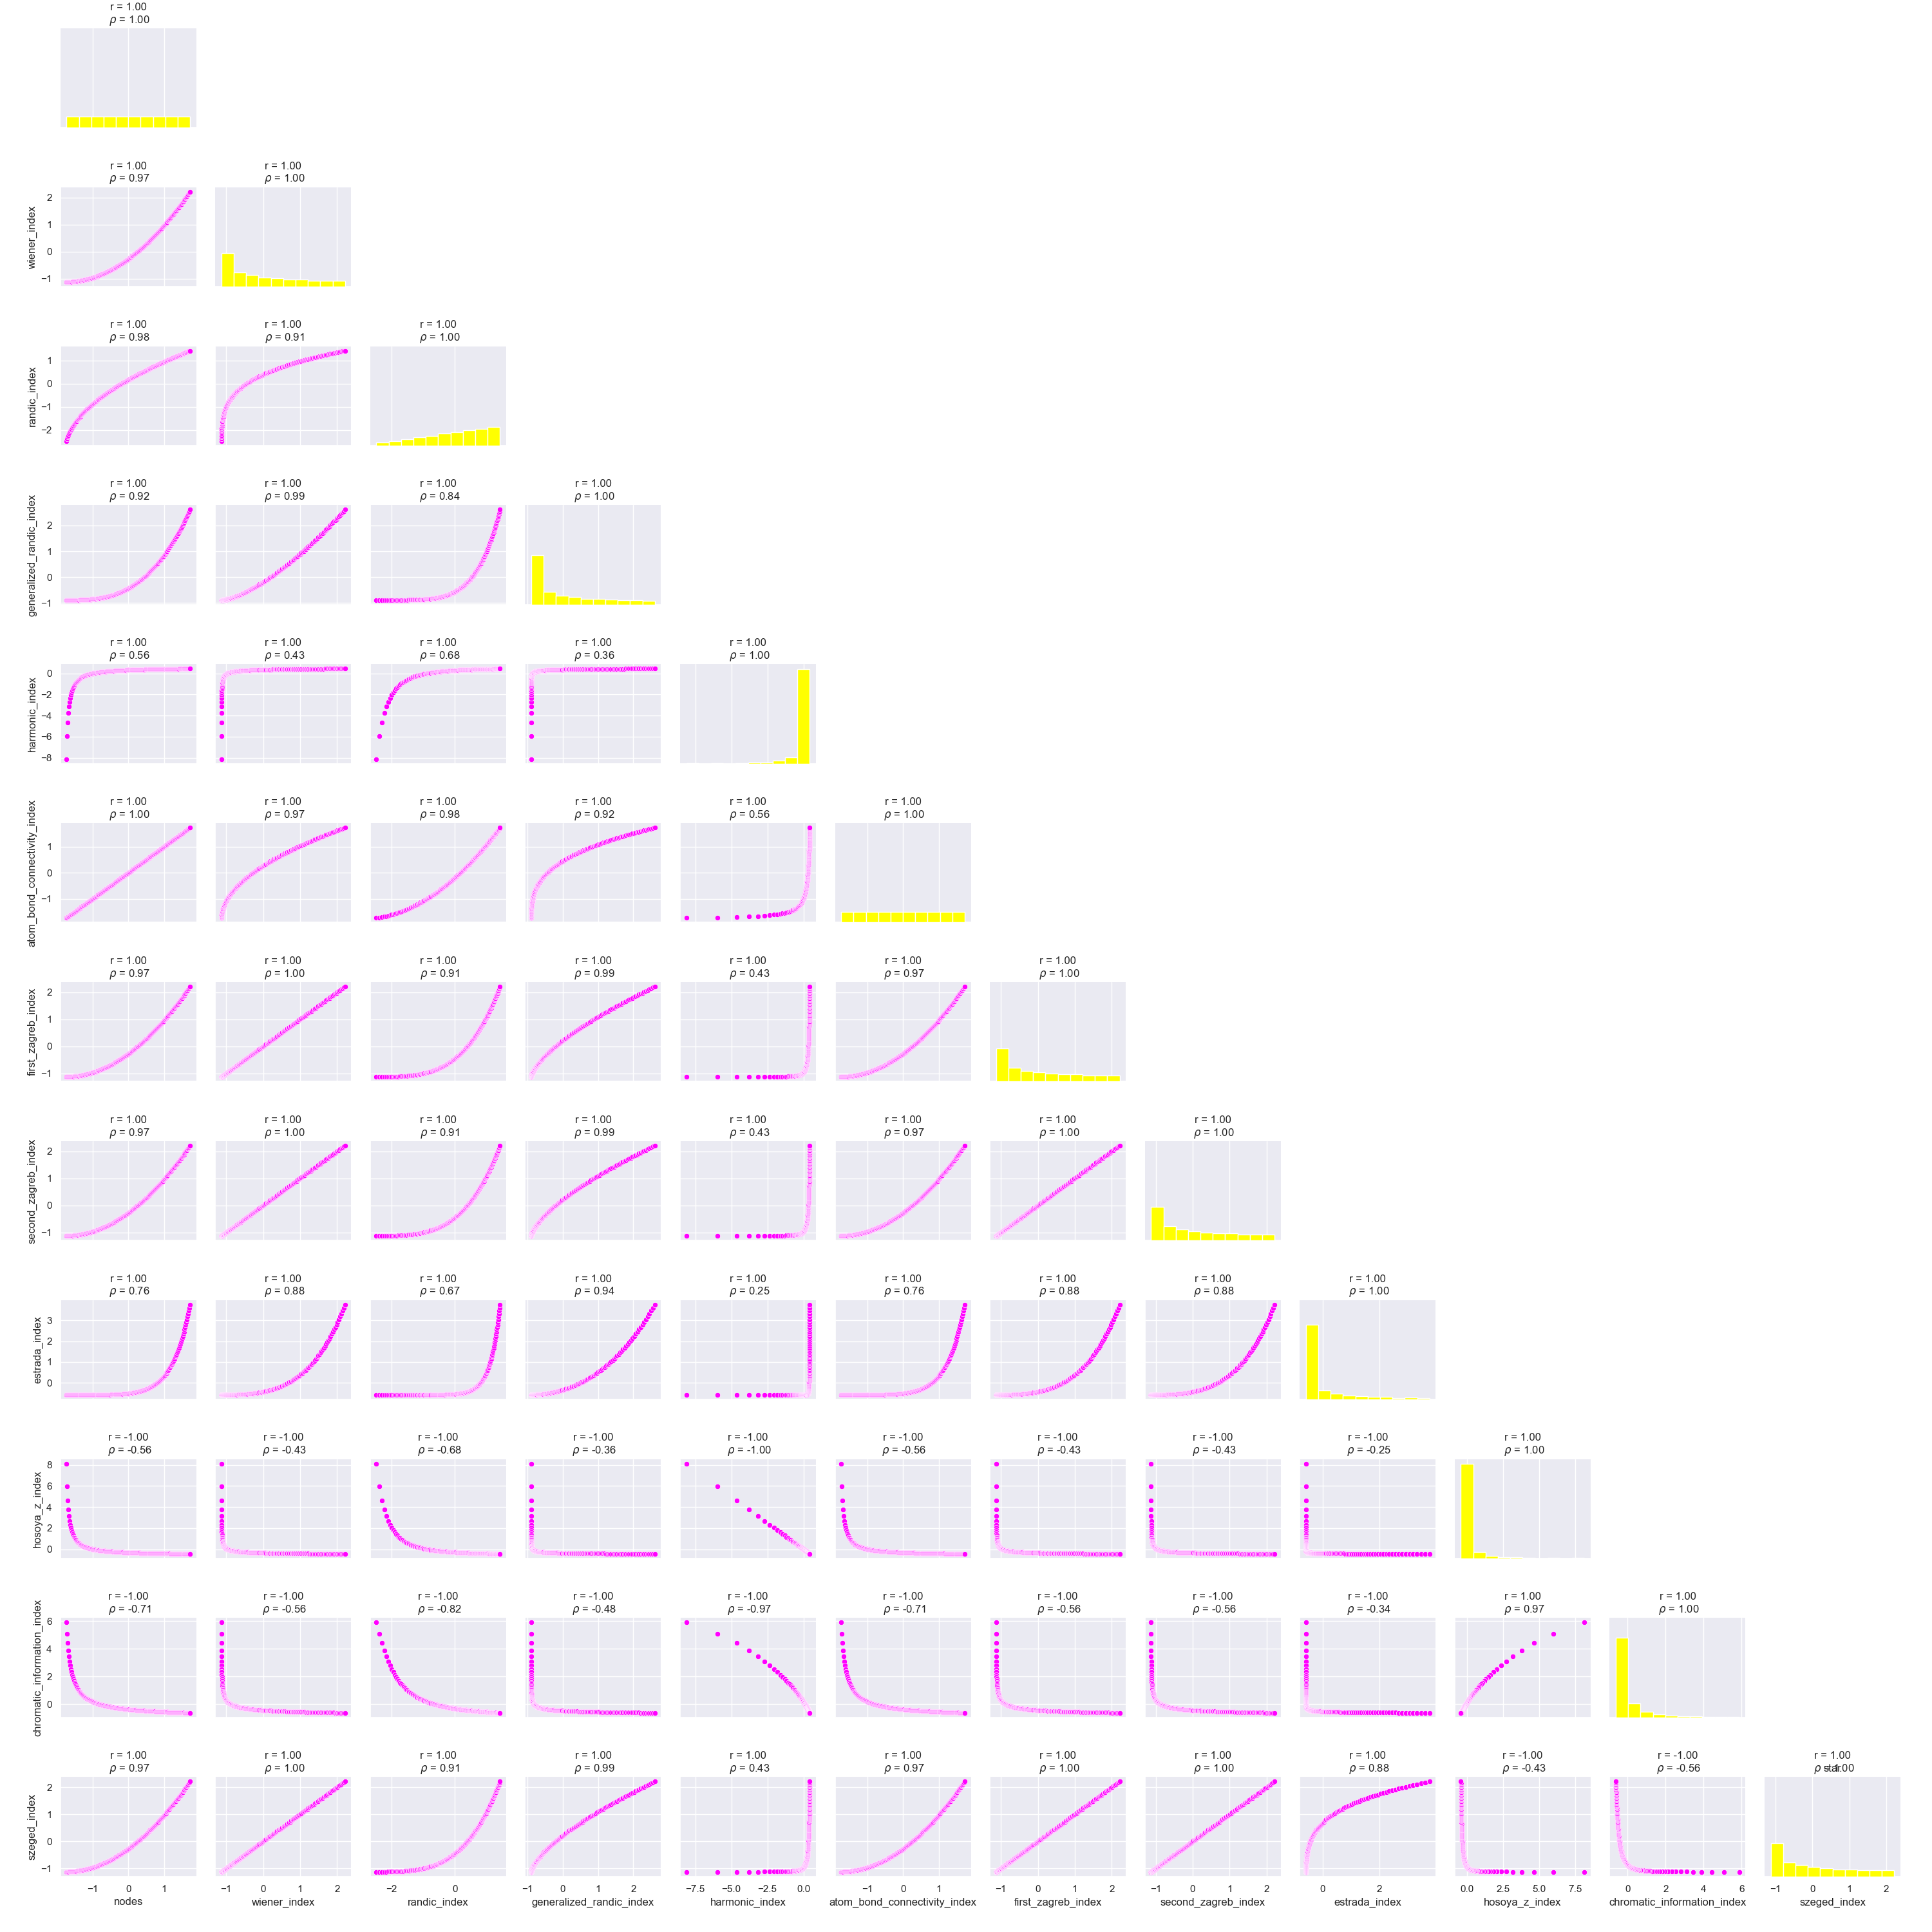
\includegraphics[width=1.2\textwidth]{images/30_results/star-correlation-pairs.png}
    \caption{Einzelne Vergleiche der topologischen Indizes der Klasse \mintinline{python3}{star}}
    \label{fig:correlation-pairs-star}
\end{figure}

\begin{landscape}
    \subsection{Einfluss aller topologischen Indizes auf die Hauptkomponenten} \label{sec:ti-pca}
    \begin{code}
        \begin{minted}[frame=lines,framesep=2mm,baselinestretch=1.2,bgcolor=LightGray,fontsize=\scriptsize,linenos]{text}   
topological_indices_all_graphs key: random, shape: 1000
------------ PCA random 4 components ------------
        wiener  randic  generalized_randic  harmonic    abc  1st zagreb  2nd zagreb  estrada      z    cii  szeged
PC-1   0.338   0.331               0.310     0.331  0.337       0.334       0.327    0.119 -0.172  0.297   0.327
PC-2   0.007  -0.165               0.303    -0.165 -0.068       0.121       0.200    0.554  0.575 -0.342   0.198
PC-3  -0.113  -0.019              -0.075    -0.019 -0.077      -0.131      -0.123    0.784 -0.544  0.128  -0.127
PC-4   0.057   0.258              -0.379     0.258  0.166      -0.103      -0.230    0.239  0.576  0.431  -0.235

topological_indices_all_graphs key: smallworld, shape: 1000
------------ PCA smallworld 4 components ------------
        wiener  randic  generalized_randic  harmonic    abc  1st zagreb  2nd zagreb  estrada      z    cii  szeged
PC-1   0.344   0.334               0.317     0.334  0.342       0.341       0.334    0.119 -0.059  0.290   0.334
PC-2  -0.034  -0.172               0.253    -0.172 -0.096       0.071       0.147    0.649  0.556 -0.298   0.143
PC-3   0.056   0.088              -0.082     0.088  0.076       0.020      -0.018   -0.537  0.813  0.134  -0.016
PC-4  -0.042   0.212              -0.351     0.212  0.072      -0.190      -0.278    0.517  0.159  0.546  -0.278

topological_indices_all_graphs key: scalefree, shape: 200
------------ PCA scalefree 4 components ------------
        wiener  randic  generalized_randic  harmonic    abc  1st zagreb  2nd zagreb  estrada      z    cii  szeged
PC-1   0.342   0.333               0.314     0.333  0.340       0.339       0.331    0.123 -0.123  0.287   0.332
PC-2   0.019  -0.151               0.279    -0.151 -0.055       0.122       0.192    0.457  0.640 -0.411   0.184
PC-3  -0.109  -0.079               0.021    -0.079 -0.105      -0.090      -0.056    0.815 -0.526  0.086  -0.064
PC-4   0.040   0.275              -0.388     0.275  0.154      -0.138      -0.260    0.323  0.511  0.395  -0.256

topological_indices_all_graphs key: complete, shape: 200
------------ PCA complete 4 components ------------
        wiener  randic  generalized_randic  harmonic    abc  1st zagreb  2nd zagreb  estrada    z    cii  szeged
PC-1   0.346   0.338               0.313     0.338  0.345       0.341       0.332    0.094  0.0  0.284   0.346
PC-2  -0.026  -0.153               0.251    -0.153 -0.085       0.070       0.144    0.879 -0.0 -0.291  -0.026
PC-3  -0.073   0.201              -0.410     0.201  0.045      -0.233      -0.326    0.459 -0.0  0.605  -0.073
PC-4   0.233   0.202              -0.550     0.202  0.271       0.036      -0.188    0.088  0.0 -0.624   0.233
    

        \end{minted}
        \newpage
        \vspace*{\fill}

        \begin{minted}[frame=lines,framesep=2mm,baselinestretch=1.2,bgcolor=LightGray,fontsize=\scriptsize,linenos]{text}   
        topological_indices_all_graphs key: line, shape: 200
------------ PCA line 4 components ------------
    wiener  randic  generalized_randic  harmonic    abc  1st zagreb  2nd zagreb  estrada      z    cii  szeged
PC-1  -0.311  -0.331              -0.331    -0.331 -0.331      -0.331      -0.331   -0.331  0.174 -0.083  -0.311
PC-2   0.179   0.024               0.025     0.025  0.024       0.024       0.024    0.024  0.611 -0.748   0.179
PC-3   0.239  -0.037              -0.036    -0.037 -0.038      -0.037      -0.037   -0.037  0.670  0.653   0.239
PC-4  -0.560   0.176               0.177     0.177  0.175       0.176       0.176    0.176  0.384  0.086  -0.560

topological_indices_all_graphs key: tree, shape: 400
------------ PCA tree 4 components ------------
    wiener  randic  generalized_randic  harmonic    abc  1st zagreb  2nd zagreb  estrada      z    cii  szeged
PC-1   0.299   0.320               0.315     0.319  0.320       0.319       0.319    0.320 -0.240  0.227   0.299
PC-2   0.328   0.034               0.054     0.031  0.040       0.047       0.047    0.040  0.588 -0.653   0.328
PC-3   0.094  -0.006              -0.053    -0.001 -0.019      -0.032      -0.032   -0.018  0.691  0.706   0.095
PC-4  -0.533   0.146               0.354     0.141  0.153       0.185       0.216    0.162  0.341 -0.136  -0.533

topological_indices_all_graphs key: star, shape: 200
------------ PCA star 4 components ------------
    wiener  randic  generalized_randic  harmonic    abc  1st zagreb  2nd zagreb  estrada      z    cii  szeged
PC-1  -0.332  -0.329              -0.321    -0.215 -0.336      -0.332      -0.332   -0.282  0.215  0.253  -0.332
PC-2   0.160  -0.094               0.222    -0.526  0.027       0.160       0.160    0.281  0.526  0.455   0.160
PC-3   0.077   0.412              -0.184    -0.235  0.347       0.079       0.077   -0.734  0.235 -0.047   0.077
PC-4  -0.197   0.434              -0.214    -0.269  0.147      -0.196      -0.197    0.485  0.269 -0.458  -0.197

        \end{minted}
        \caption{Ausgabe aller Komponenten der vier Hauptkomponenten der verschiedenen Netzwerk-Klassen}
        \vspace*{\fill}
    \end{code}
\end{landscape}

\subsection{Erklärbare Varianzen und Usefulness-Scores aller Indizes} \label{sec:all_pca}
\begin{code}
    \begin{minted}[frame=lines,framesep=2mm,baselinestretch=1.2,bgcolor=LightGray,fontsize=\scriptsize,linenos]{text}   
topological_indices_all_graphs key: random, shape: 1000
------------ PCA random 4 explained variance ratio ------------
        explained variance ratio
PC-1                     0.784
PC-2                     0.116
PC-3                     0.069
PC-4                     0.026
------------ PCA random combined usefulness score ------------
                    usefulness score
wiener                     0.747183
randic                     0.899278
generalized_randic         0.985581
harmonic                   0.899467
abc                        0.833882
1st zagreb                 0.915968
2nd zagreb                 0.998606
estrada                    0.000000
z                          0.476098
cii                        0.985445
szeged                     1.000000

topological_indices_all_graphs key: smallworld, shape: 1000
------------ PCA smallworld 4 explained variance ratio ------------
        explained variance ratio
PC-1                     0.760
PC-2                     0.103
PC-3                     0.084
PC-4                     0.048
------------ PCA smallworld combined usefulness score ------------
                    usefulness score
wiener                     0.831004
randic                     0.985409
generalized_randic         1.000000
harmonic                   0.985451
abc                        0.898649
1st zagreb                 0.882126
2nd zagreb                 0.940025
estrada                    0.432969
z                          0.000000
cii                        0.977841
szeged                     0.936464

topological_indices_all_graphs key: scalefree, shape: 200
------------ PCA scalefree 4 explained variance ratio ------------
        explained variance ratio
PC-1                     0.765
PC-2                     0.121
PC-3                     0.076
PC-4                     0.033
------------ PCA scalefree combined usefulness score ------------
                    usefulness score
wiener                     0.766124
randic                     0.985386
generalized_randic         0.984622
harmonic                   0.985271
abc                        0.861029
1st zagreb                 0.937208
2nd zagreb                 1.000000
estrada                    0.000000
z                          0.092939
cii                        0.989833
szeged                     0.999622

topological_indices_all_graphs key: complete, shape: 200
------------ PCA complete 4 explained variance ratio ------------
        explained variance ratio
PC-1                     0.830
PC-2                     0.104
PC-3                     0.057
PC-4                     0.008
------------ PCA complete combined usefulness score ------------
                    usefulness score
wiener                     0.942523
randic                     0.987024
generalized_randic         1.000000
harmonic                   0.987024
abc                        0.955097
1st zagreb                 0.967715
2nd zagreb                 0.990307
estrada                    0.627966
z                          0.000000
cii                        0.974817
szeged                     0.942523

topological_indices_all_graphs key: line, shape: 200
------------ PCA line 4 explained variance ratio ------------
        explained variance ratio
PC-1                     0.822
PC-2                     0.121
PC-3                     0.041
PC-4                     0.016
------------ PCA line combined usefulness score ------------
                    usefulness score
wiener                     1.000000
randic                     0.848306
generalized_randic         0.848312
harmonic                   0.848308
abc                        0.848286
1st zagreb                 0.848303
2nd zagreb                 0.848307
estrada                    0.848304
z                          0.584325
cii                        0.000000
szeged                     1.000000

topological_indices_all_graphs key: tree, shape: 400
------------ PCA tree 4 explained variance ratio ------------
        explained variance ratio
PC-1                     0.885
PC-2                     0.072
PC-3                     0.028
PC-4                     0.013
------------ PCA tree combined usefulness score ------------
                    usefulness score
wiener                     0.999889
randic                     0.617134
generalized_randic         0.661762
harmonic                   0.598685
abc                        0.649556
1st zagreb                 0.686914
2nd zagreb                 0.692432
estrada                    0.651624
z                          0.305157
cii                        0.000000
szeged                     1.000000

topological_indices_all_graphs key: star, shape: 200
------------ PCA star 4 explained variance ratio ------------
        explained variance ratio
PC-1                     0.779
PC-2                     0.193
PC-3                     0.024
PC-4                     0.003
------------ PCA star combined usefulness score ------------
                    usefulness score
wiener                 7.190176e-01
randic                 4.641530e-01
generalized_randic     1.000000e+00
harmonic               2.433945e-15
abc                    7.673370e-03
1st zagreb             7.173088e-01
2nd zagreb             7.190176e-01
estrada                7.781882e-01
z                      0.000000e+00
cii                    5.466071e-01
szeged                 7.190176e-01


    \end{minted}
    \caption{Ausgabe aller erklärbaren Varianzen und Usefulness-Scores aller Indizes}
\end{code}

\subsection{Weights and Biases Dashboard für die Visualisierung der Ergebnisse} \label{sec:wandb_dashboard}

\begin{figure}[ht]
    \centering
    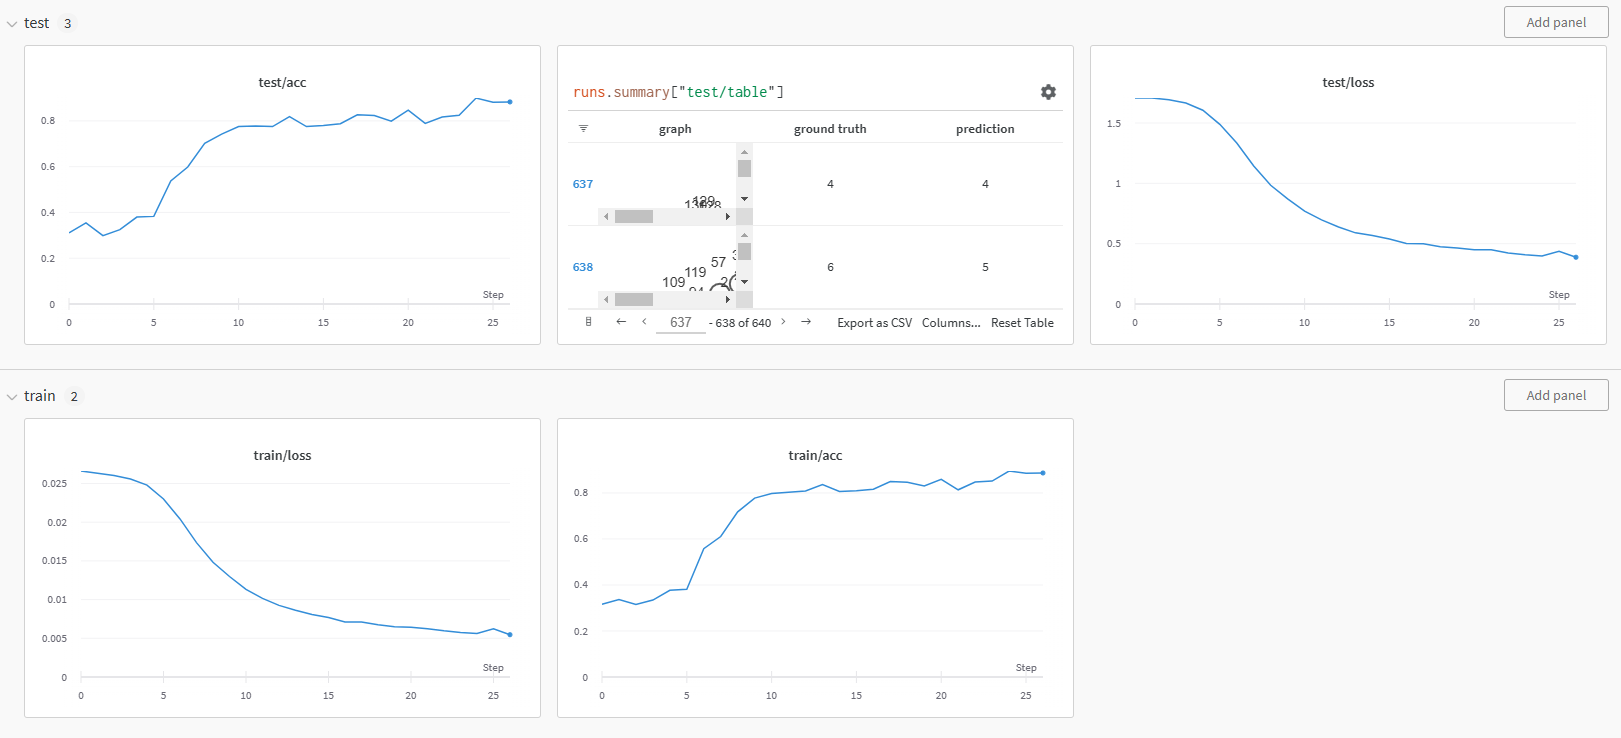
\includegraphics[width=0.9\textwidth]{images/30_results/wandb_dashboard.png}
    \caption{Weights and Biases Dashboard für die Visualisierung der Ergebnisse}
    \label{fig:wandb_dashboard}
\end{figure}

\listoffigures

\listoftables

\listoftheorems[title={Definitionsverzeichnis}]

\listoflistings

\bibliographystyle{ieeetr}
\bibliography{sources}
%\nocite{*}

\chapter*{Selbstständigkeitserklärung}
Ich erkläre hiermit, dass ich diese Thesis selbstständig verfasst
und keine anderen als die angegebenen Quellen benutzt habe.
Alle Stellen, die wörtlich oder sinngemäss aus Quellen entnommen wurden,
habe ich als solche kenntlich gemacht. Ich versichere zudem, dass ich bisher
noch keine wissenschaftliche Arbeit mit gleichem oder ähnlichem Inhalt an der
Fernfachhochschule Schweiz oder an einer anderen Hochschule eingereicht habe.
Mir ist bekannt, dass andernfalls die Fernfachhochschule Schweiz zum Entzug
des aufgrund dieser Thesis verliehenen Titels berechtigt ist.

\vspace{4cm}
\noindent
Zürich, 15. März 2023
\hrule \ \\[-0.5ex]

\vspace*{-3.2cm}\hspace*{4cm}\makebox[0pt][l]{%
    \raisebox{-\totalheight}[0pt][0pt]{%
        
\includegraphics[scale=0.5]{images/99_appendix/signature.png}
    }
}

\unskip
\vspace{2cm}
Ort, Datum, Unterschrift
